\documentclass[aspectratio=169]{beamer}
%\setbeamertemplate{footline}[frame number]
\usepackage{color,amsmath}
\usepackage{subfigure}
\usepackage{booktabs}
\usepackage{framed}
\usepackage{comment}
\hypersetup{
colorlinks=true,
linkcolor=blue,
filecolor=magenta,      
urlcolor=blue,
pdftitle={Overleaf Example},
pdfpagemode=FullScreen}
\usepackage{tabularx}

%%%%%%%%%%%%%%%%%%%%%%%%%%
\title[]{Survey research in the digital age}
\author[]{Bernhard Clemm von Hohenberg\\Department of Computational Social Science\\GESIS}
\date[]{Summer Institutes in Computational Social Science\\July 28, 2023}
\begin{document}
%%%%%%%%%%%%%%%%%%%%%%%%%%
\frame{\titlepage}
%%%%%%%%%%%%%%%%%%%%%%%%%%

\begin{frame}{Schedule}

\vspace{0.5em}
\begin{itemize}
\item 9.00-9.45 Introduction \& total error survey framework
\item \textcolor{violet}{9.45-10.15 Probability and non-probability sampling}
\vspace{0.5em}
\item Coffee break
\vspace{0.5em}
\item 10.30-11.00 Computer-administered interviewing
\item 11.00-11.30 Linking surveys to big data
\item 11:30-13:00 Intro and begin group exercise
\vspace{0.5em}
\item Lunch (or Eisbach plunge)
\vspace{0.5em}
\item 14:00-15:45 Continue group exercise
\end{itemize}

\end{frame}
%%%%%%%%%%%%%%%%%%%%%%%%%%%
\begin{frame}{Schedule}
\begin{center}
\renewcommand{\arraystretch}{1.5}
\begin{tabular}{p{0.1\textwidth}p{0.26\textwidth}p{0.24\textwidth}p{0.24\textwidth}}
& \textbf{Sampling} & \textbf{Interviews} & \textbf{Data environment}\\
\hline \hline
1st era & Area probability & Face-to-face & Stand-alone \\
\hline
2nd era & Random digital dial probability & Telephone & Stand-alone \\
\hline
3rd era & \textcolor{violet}{Non-probability} & Computer-administered  & Linked \\
\end{tabular}
\end{center}

\end{frame}
%%%%%%%%%%%%%%%%%%%%%%%%%%%
\begin{frame}{Warm-up exercise}

Go to \url{https://forms.gle/AtdDu6hS8RiuhUWB6} and indicate your height in cm (e.g., ``194'') and your sex. If you don't know your height, or don't want to tell, give an estimate or some plausible number. 

\end{frame}
%%%%%%%%%%%%%%%%%%%%%%%%%%%
\begin{frame}{Warm-up exercise}

Let's have a look at 

\begin{itemize}
    \item ... the average height of the population (all of you)
    \item ... the average height estimated from a random sample
    \item ... the average height estimated from a non-random (but probability) sample
\end{itemize}

\end{frame}

%%%%%%%%%%%%%%%%%%%%%%%%%
\begin{frame}{Probability samples}

\begin{itemize}
\item Probability sample (roughly): every unit from a frame population has a known and non-zero probability of inclusion
\pause
\begin{itemize}
\item In the case of a simple random sample, this inclusion probability is $n/N$, with $n$ being the sample size and $N$ being size of population
\end{itemize}
\pause
\item In practice, we rarely deal with a simple random sample
\item However, if we know the inclusion probability, we can get an unbiased estimate of the population mean.
\end{itemize}

\end{frame}

%%%%%%%%%%%%%%%%%%%%%%%%%%
\begin{frame}{Probability-based estimation}

Horvitz-Thompson estimator: the estimator for the population mean $\bar{y}$ is

$$\hat{\bar{y}} = \frac{1}{N}\sum_{i \in s}\frac{y_i}{\pi_i}$$

where $\pi_i$ is person $i$'s probability of inclusion. Verbally, this is a weighted sample mean where the weights are inversely related to the probability of selection.

\end{frame}

%%%%%%%%%%%%%%%%%%%%%%%%%
\begin{frame}{Theory vs. practice}

\begin{columns}

\begin{column}{0.32\textwidth}
\textbf{Inference from probability samples in theory} \\
\vspace{5.5em}
known information about sampling \\
+ respondents \\
= estimates
\end{column}
\pause
\begin{column}{0.32\textwidth}
\textbf{Inference from probability samples in practice}
\vfill
\vspace{0.5em}
auxiliary information \\
+ assumptions \\
= estimated information about sampling \\
\vspace{0.5em}
estimated information about sampling \\
+ respondents \\
= estimates
\end{column}
\pause
\begin{column}{0.32\textwidth}
\textbf{Inference from non-probability samples in practice}
\vfill
\vspace{0.5em}
auxiliary information \\
+ assumptions \\
= estimated information about sampling \\
\vspace{0.5em}
estimated information about sampling \\
+ respondents \\
= estimates
\end{column}

\end{columns}

\end{frame}
%%%%%%%%%%%%%%%%%%%%%%%%%
\begin{frame}{Theory vs. practice}

$$\hat{\bar{y}} = \frac{1}{N}\sum_{i \in s}\frac{y_i}{\hat{\pi}_i}$$

where $\hat{\pi}_i = \frac{n_g}{N_g} \quad \forall \quad i \in g$ (estimated probability of inclusion)

\vfill

Requires:
\begin{itemize}
\item auxiliary information $(N_g)$
\item ability to place respondents in groups
\item assumptions
\end{itemize}

\end{frame}
%%%%%%%%%%%%%%%%%%%%%%%%
\begin{frame}{Theory vs. practice}

\begin{itemize}
\item 
Not all probability samples look like miniature versions of the population---but, with appropriate weighting, probability samples can yield unbiased estimates
\pause
\item How you collect your data impacts how you make inference
\pause
\item Key to many adjustment methods is to use external information and make assumptions
\pause
\item If external information is incorrect or assumptions are wrong, then you can make things worse (but it usually seems to make things better)
\end{itemize}

\end{frame}
%%%%%%%%%%%%%%%%%%%%%%%%%%
\begin{frame}{Back to warm-up}

Back to the average height of your group:

\begin{itemize}
    \item If I know the inclusion probability (e.g., 0.8 for males, 0.2 for females), it does not matter that the sample is non-probability
    \item If I know the frequency of males/females in the population (e.g., 0.5/0.5), I can build a weighted average (0.5*average males + 0.5*average females)
    \item However, I often don't know \textit{why} more males participated than females; if I see more males than females in my sample, I have to \textit{assume} that this imbalance is caused by \textit{sex} and not something else
\end{itemize}

\end{frame}
%%%%%%%%%%%%%%%%%%%%%%%%%%
\begin{frame}

\begin{center}
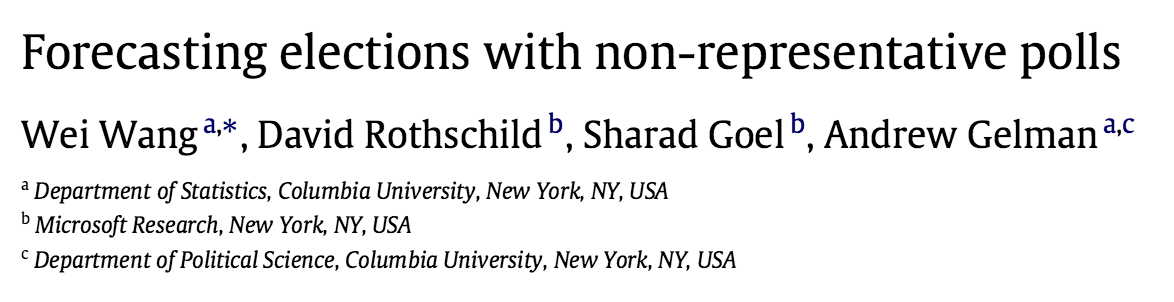
\includegraphics[width=0.8\textwidth]{figures/wang_forecasting_2015_title}
\end{center}

\begin{center}

\includegraphics[width=0.4\textwidth]{figures/xboxlogo}
\end{center}

\TINY{\url{https://www.journals.elsevier.com/international-journal-of-forecasting/editors-choice-articles/forecasting-elections-with-non-representative-polls}}

\end{frame}
%%%%%%%%%%%%%%%%%%%%%%%%%%%
\begin{frame}

\begin{center}
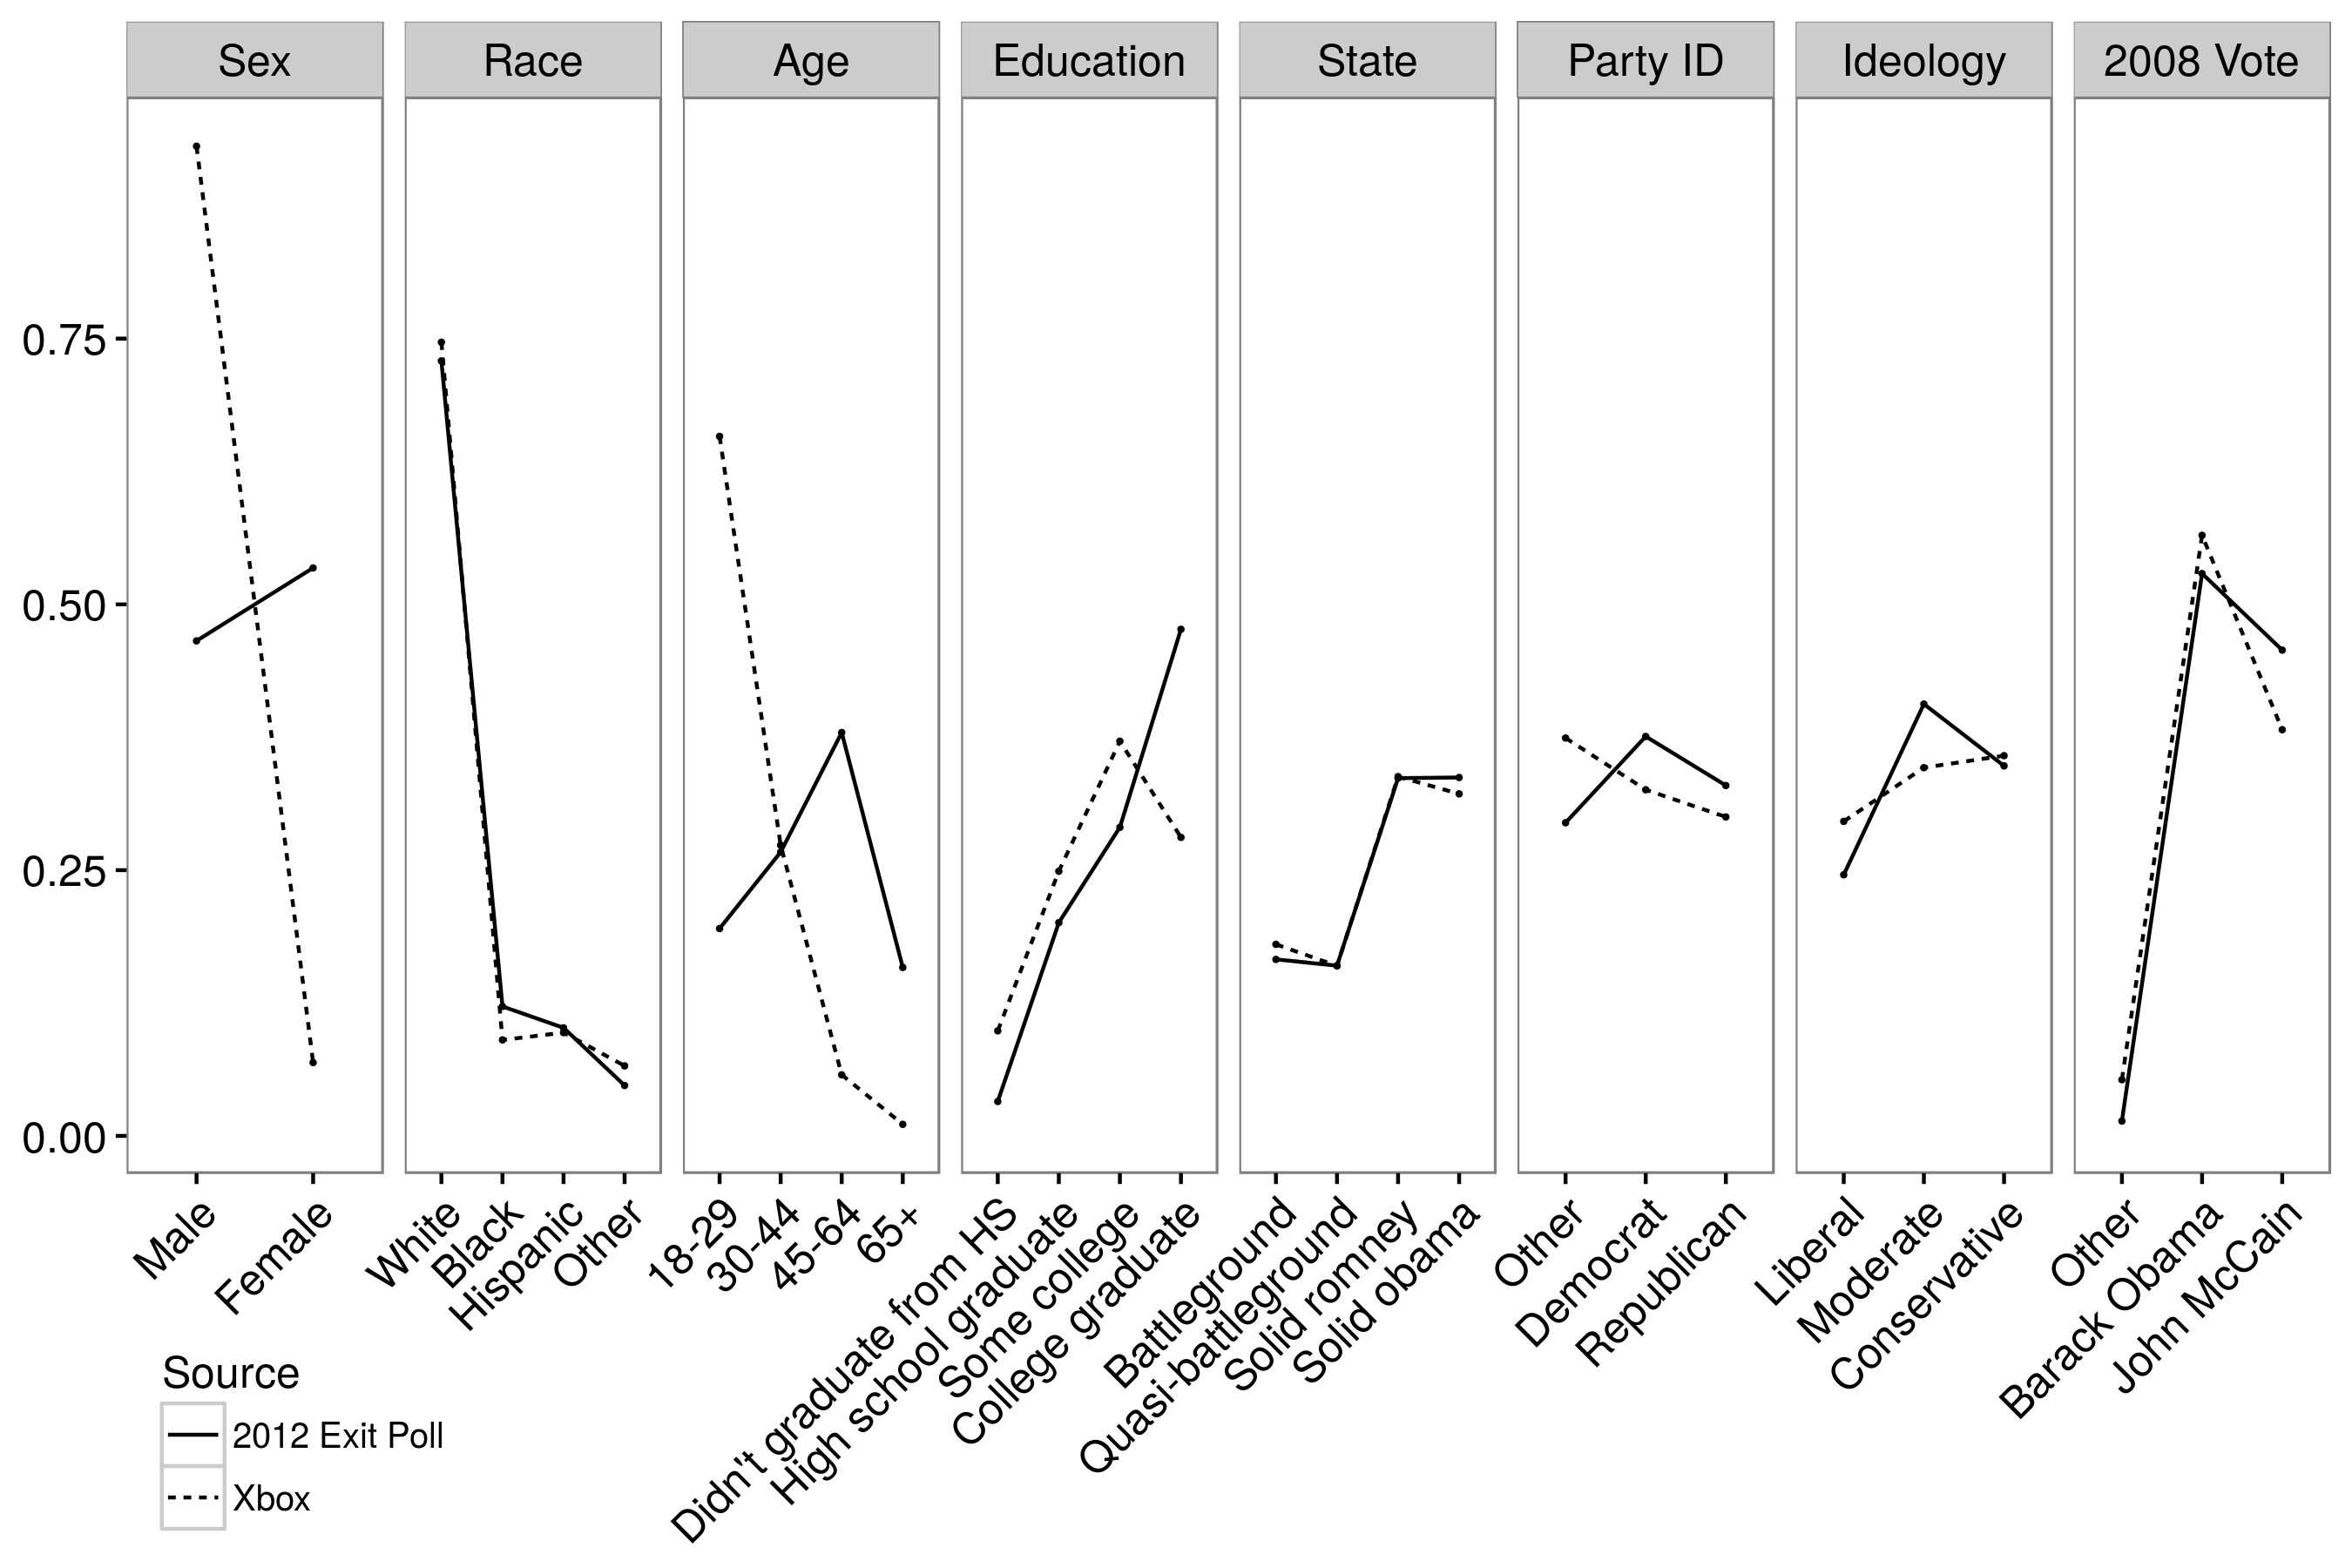
\includegraphics[width=0.55\textwidth]{figures/bitbybit3-7_wang_forecasting_2015_fig1}
\end{center}

\begin{itemize}
\item about 750,000 interviews
\item about 350,000 unique respondents
\end{itemize}

\end{frame}
%%%%%%%%%%%%%%%%%%%%%%%%%%%
\begin{frame}

\begin{center}
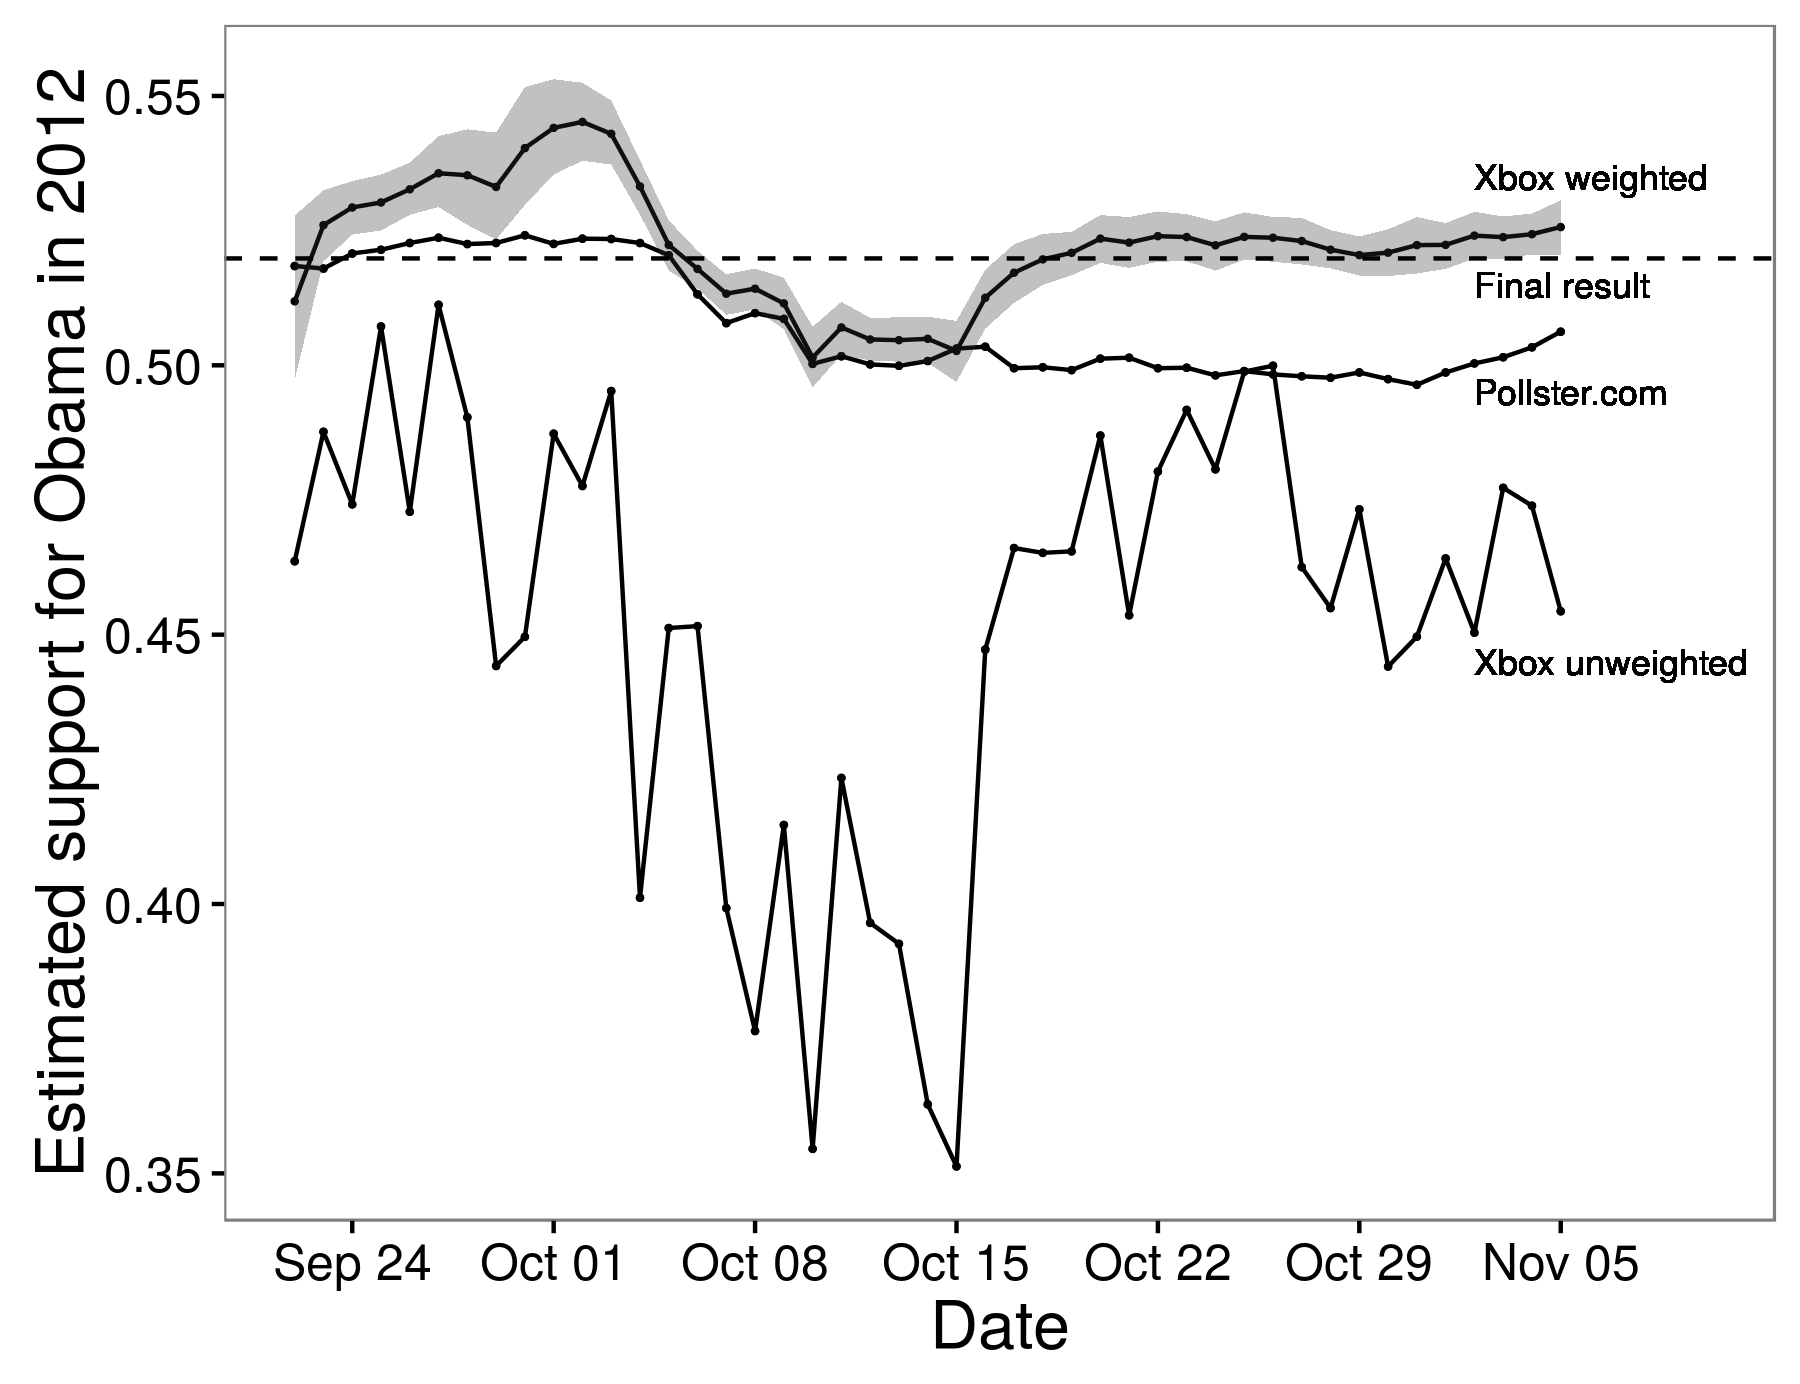
\includegraphics[width=0.7\textwidth]{figures/bitbybit3-8_wang_forecasting_2015_fig2_and_3}
\end{center}

\end{frame}
%%%%%%%%%%%%%%%%%%%%%%%%%%%
\begin{frame}

\begin{center}
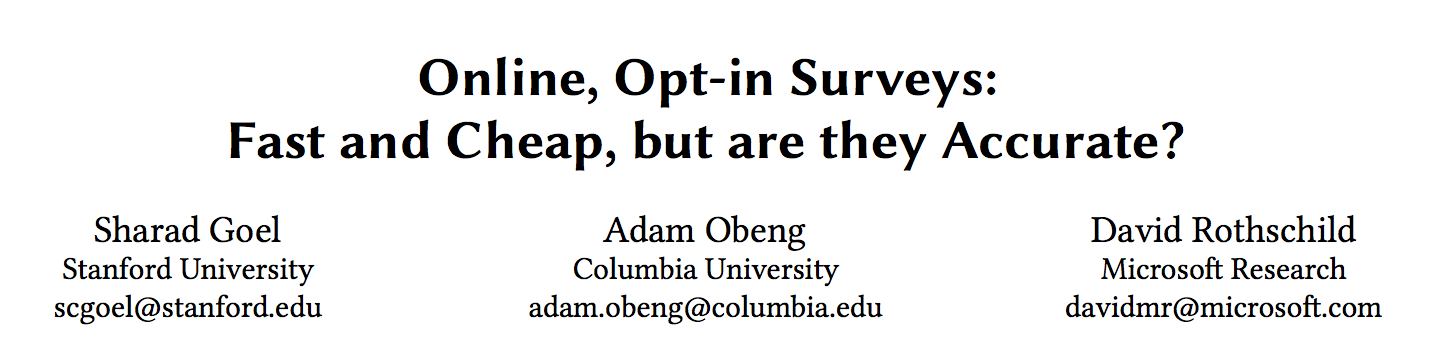
\includegraphics[width=0.9\textwidth]{figures/goel_online_2017_title}
\end{center}

\vfill
\TINY{\url{https://5harad.com/papers/dirtysurveys.pdf}}

\end{frame}
%%%%%%%%%%%%%%%%%%%%%%%%%%%
\begin{frame}{The future}

\begin{center}
... according to Matt Salganik
\vfill
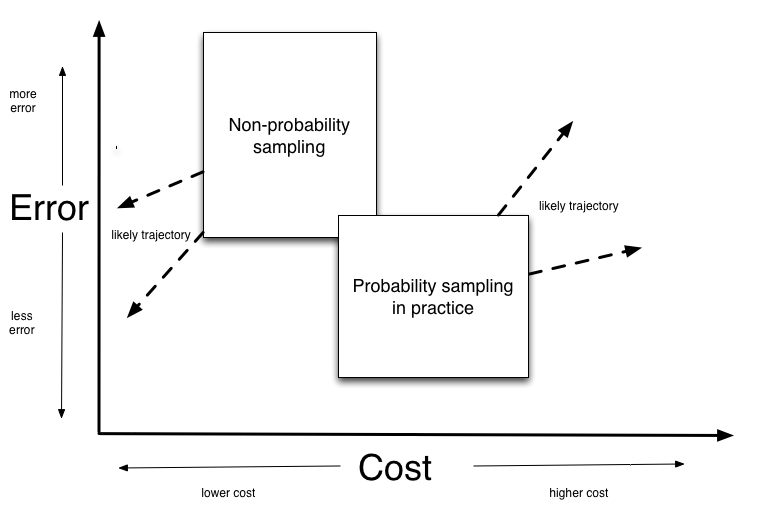
\includegraphics[width=0.7\textwidth]{figures/future_sampling}
\end{center}

\end{frame}
%%%%%%%%%%%%%%%%%%%%%%%%%%%
\begin{frame}{The future}

\begin{columns}[T]

\begin{column}{0.59\textwidth}
\begin{center}
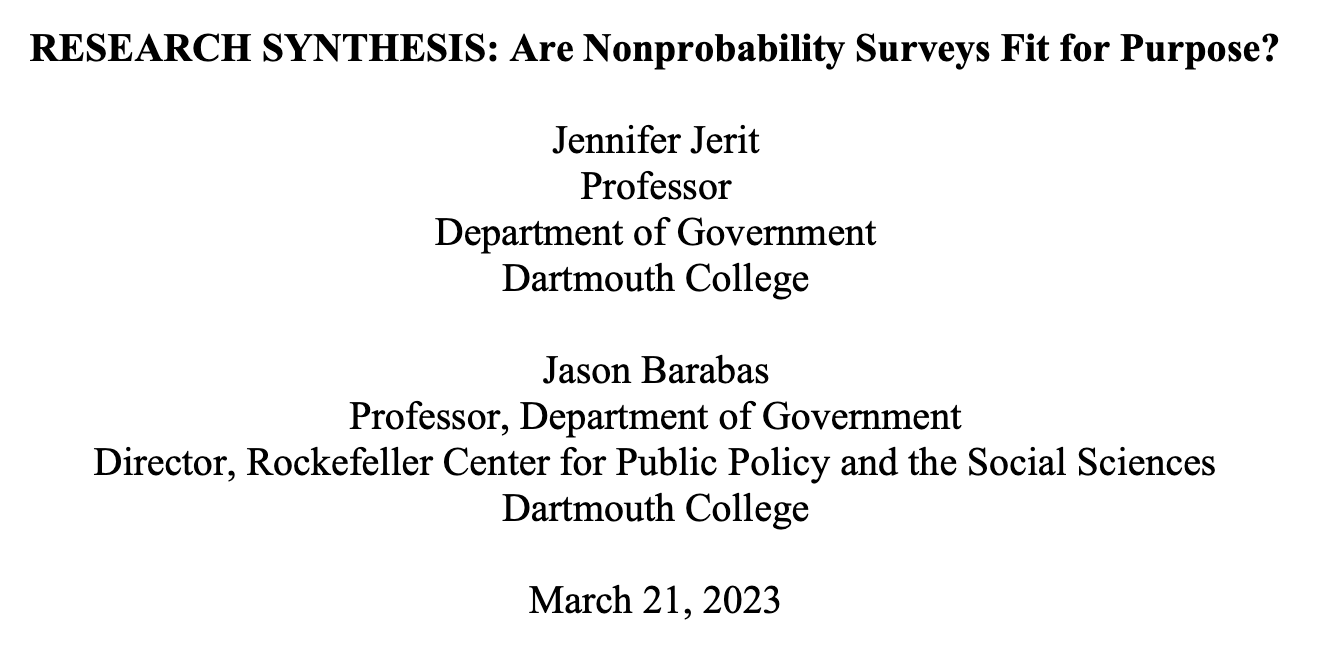
\includegraphics[width=\textwidth]{figures/jerit-barabas-abstract.png}
\end{center}
\end{column}

\begin{column}{0.39\textwidth}
\vspace{1.5em}
``In studies comparing the accuracy of probability and nonprobability samples in relation to government records, the former consistently outperforms the latter'' \\
\vspace{1.5em}
\TINY{\url{https://bpb-us-e1.wpmucdn.com/sites.dartmouth.edu/dist/d/2388/files/2023/05/JeritBarabas_NPS_Mar2023-1.pdf}}

\end{column}

\end{columns}

\end{frame}
%%%%%%%%%%%%%%%%%%%%%%%%%%%
%%%%%%%%%%%%%%%%%%%%%%%%%%%
\begin{frame}{The future}

\begin{columns}[T]

\begin{column}{0.39\textwidth}
\vspace{1.5em}
``Despite substantial drops in response rates since a prior comparison, the probability samples interviewed by telephone or the internet were the most accurate. Internet surveys of a probability sample combined with an opt-in sample were less accurate; least accurate were internet surveys of opt-in panel samples.'' \\
\vspace{1.5em}
\TINY{\url{https://academic.oup.com/poq/article-abstract/82/4/707/5151369}}
\end{column}

\begin{column}{0.59\textwidth}
\begin{center}
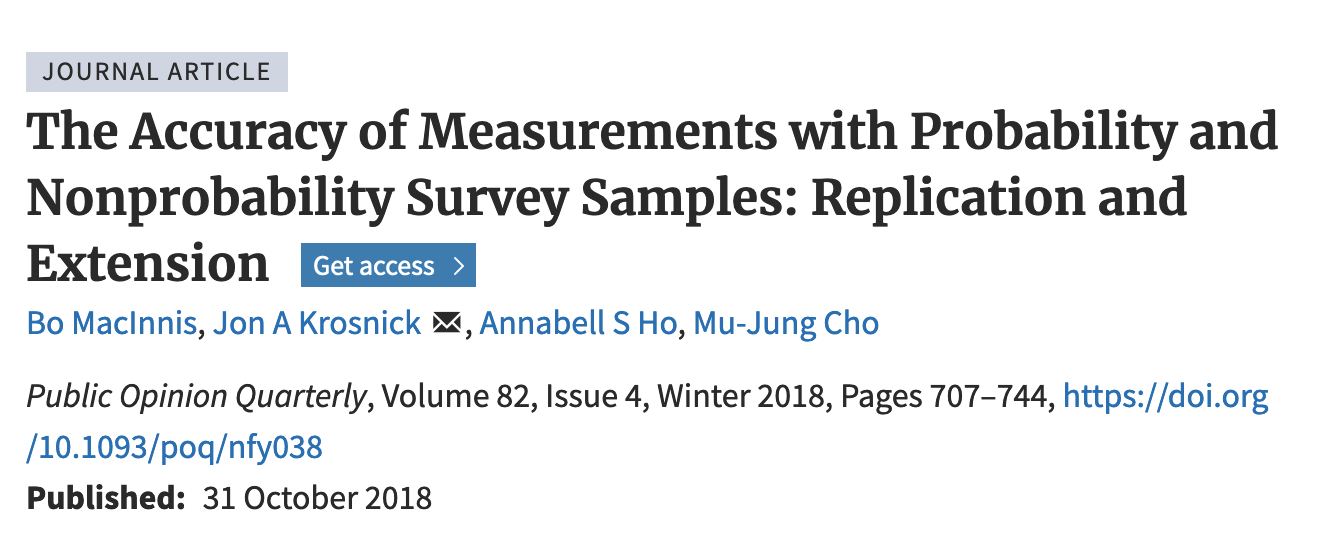
\includegraphics[width=\textwidth]{figures/maciniss-et-al-abstract.png}
\end{center}
\end{column}

\end{columns}

\end{frame}
%%%%%%%%%%%%%%%%%%%%%%%%%%%
\begin{frame}{Summary}

\begin{itemize}
\item Samples don't need to look like mini-populations
\pause
\item Key to making good estimates is for estimation process to account for the sampling process
\pause
\item There is not a bright-line difference between probability sampling in practice and non-probability sampling
\pause
\item However, still a lot of debate about how non-probability samples really perform
\end{itemize}

\end{frame}
%%%%%%%%%%%%%%%%%%%%%%%%%%%%%%
\begin{frame}

\begin{center}
\Large Questions
\end{center}

\end{frame}
%%%%%%%%%%%%%%%%%%%%%%%%%%%%%%

\end{document}